\documentclass[a4paper,french]{paper}
\usepackage{../../../../../_assets/latex/5N_OPTO_ELEC}

%Informations about this document 
%------------------------------------------
\def\module{Opto-Electronique - S5}
\def\moduleAbrege{5N-027-SCI / OptoElec}
\def\annee{}

\def\titre{Séance 1 / Bases et amplificateur linéaire}
\author{Julien VILLEMEJANE}

\subtitle{Séance 1}
\institution{LEnsE / Institut d'Optique Graduate School}

\title{\titre}
\begin{document} 
%Beginning First Page. 
%------------------------------------------
\enteteThematiqueObligatoire{}

\textit{Pour ce TD, on pourra s'appuyer sur les fiches résumées} :  \href{https://lense.institutoptique.fr/ressources/Annee1/Electronique/fiches/2020_FR_Fondamentaux.pdf}{Fondamentaux} et \href{https://lense.institutoptique.fr/ressources/Annee1/Electronique/fiches/2021_FR_ALI.pdf}{Ampli Linéaire Intégré}.

%Beginning Content. 
%------------------------------------------

%%%%%%%%%%%%%%%%%%%
%%%%%%%%%%%%%%%%%%%
\encadreTDExo{1.1 - Abaisser une tension}{
Proposez un circuit permettant d'abaisser une tension d'un facteur $k$.

$0 < k < 1$ 
}

%%%%%%%%%%%%%%%%%%%
%%%%%%%%%%%%%%%%%%%
\encadreTDExo{1.2 - Courants et tensions}{

Soit le circuit suivant :


\begin{center}
\begin{circuitikz}
\draw (0,0) to[I, l=$I_{PHD}$, invert] (0,3)
	to[short, -*, i=$I_{PHD}$] (2,3)
	to[R, R=$Z_{PHD}$, -*] (2,0)
	to[short] (0,0);
	
\draw (1,0) to[short, *-] (1,0) node[ground] {};
\draw (2,3) to[short, -*] (4,3) to[R, R=$R_{PHD}$, -*] (4, 0)
	-- (2,0);

\draw (4,3) to[short, -*] (6,3) to[R, R=$R_{e}$, -*] (6, 0)
	-- (4,0);

\draw (6,3) -- (8,3) to[R, R=$Z_{e}$] (8,0) -- (6,0);

\draw (1.2,0.3) edge[->, color={red}] (1.2,2.7);
	\node[text={red}] (Vs) at (0.9,1.5){$V_s$}; 

\end{circuitikz}
\end{center}

\begin{enumerate}
	\item Donnez l'expression de $V_S$ en fonction de $I_{PHD}$.
	\item Que devient cette expression si $R_e \longrightarrow +\infty$, $Z_e \longrightarrow +\infty$ et $Z_{PHD} \longrightarrow +\infty$ ?
	
	\medskip 
	
	On se place à présent en régime harmonique.
	
	$Z_{PHD} $ est une capacité $C_{PHD} $ et $Z_e$ est une capacité $C_e$.
	
	\item Que devient l'expression de $V_S$ en fonction de $I_{PHD}$ ?
	\item A quoi peuvent correspondre l'ensemble des éléments du montage ?
	
\end{enumerate}
}

%%%%%%%%%%%%%%%%%%%
%%%%%%%%%%%%%%%%%%%
\encadreTDExo{1.3 - Amplificateur linéaire intégré}{
On fournit en annexe une partie de la documentation technique de l'amplificateur linéaire intégré (ALI) \textbf{TL081}.

\begin{enumerate}
	\item Cherchez dans la documentation les valeurs des paramètres électriques suivants :
	\begin{enumerate}
		\item Tension d'alimentation (Supply Voltage)
		\item Tension d'entrée différentielle maximale
		\item Amplification différentielle 
		\item Gain unitaire ou produit gain-bande-passante
		\item Impédance d'entrée 
		\item Slew Rate
	\end{enumerate}
	\item Précisez à quoi correspondent ces paramètres.
	\item Rappelez la relation entre les entrées $V^+$, $V^-$ et la sortie $V_S$ d'un ALI.
	\item Tracez la caractéristique $V_S = f (\varepsilon)$ où $\varepsilon = (V^+ - V^-)$ pour cet ALI avec $V_{CC} = 15\operatorname{V}$.
	\item Est-ce un bon amplificateur ? Quelle est sa bande-passante ?

\end{enumerate}
}

%%%%%%%%%%%%%%%%%%%
%%%%%%%%%%%%%%%%%%%
\encadreTDExo{1.4 - Amplificateur inverseur}{
On se propose d'étudier à présent le montage suivant :

\begin{center}
\begin{circuitikz} 
	\node [op amp, fill=blue!10!white](A1) at (0,0){\texttt{AOP1}};
	\draw (A1.-) to[short] ++(-.5,0) coordinate(A) to[short] ++(0,1.5) coordinate(B) to[R=$R_2$] (B -| A1.out) to[short, -*] (A1.out);
	\draw (A1.-) to[short,-*] ++(-.5,0) coordinate(AA) to[R=$R_1$] ++(-2.5,0) coordinate(BB) to[short,-o] ++(-.5,0) coordinate(CC);
	\draw (A1.+) to[short] ++(0,-0.5) node[ground]{};
	\draw (A1.out) to[short,-o] ++(1,0) coordinate(D);
	\draw (-4.6,-1) edge[->,color={green!40!black}] (-4.6,0.3);
	\node[text={green!40!black}] (Ve) at (-5.1,-0.35){$V_e$}; 
	\draw (-4.6,-1.3)  to[open,-o] ++(0,0) node[ground](GND){};
	\draw (2.2,-1) edge[->, color={red}] (2.2,-0.3);
	\node[text={red}] (Vs) at (1.7,-0.6){$V_s$}; 
	\draw (2.2,-1.3)  to[open,-o] ++(0,0) node[ground](GND){};
	
\end{circuitikz}
\end{center}

\begin{enumerate}
	\item Donnez la relation entre $V_S$ et $V_E$ du circuit précédent en utilisant la relation d'entrées-sortie standard d'un ALI.
	\item Quelle hypothèse fait-on souvent lorsqu'on utilise des ALI avec une rétroaction négative ?
	\item Quelle relation trouve-t-on alors entre $V_S$ et $V_E$ en partant de cette hypothèse ?
	\item Cette hypothèse est-elle justifiée ?
\end{enumerate}

}

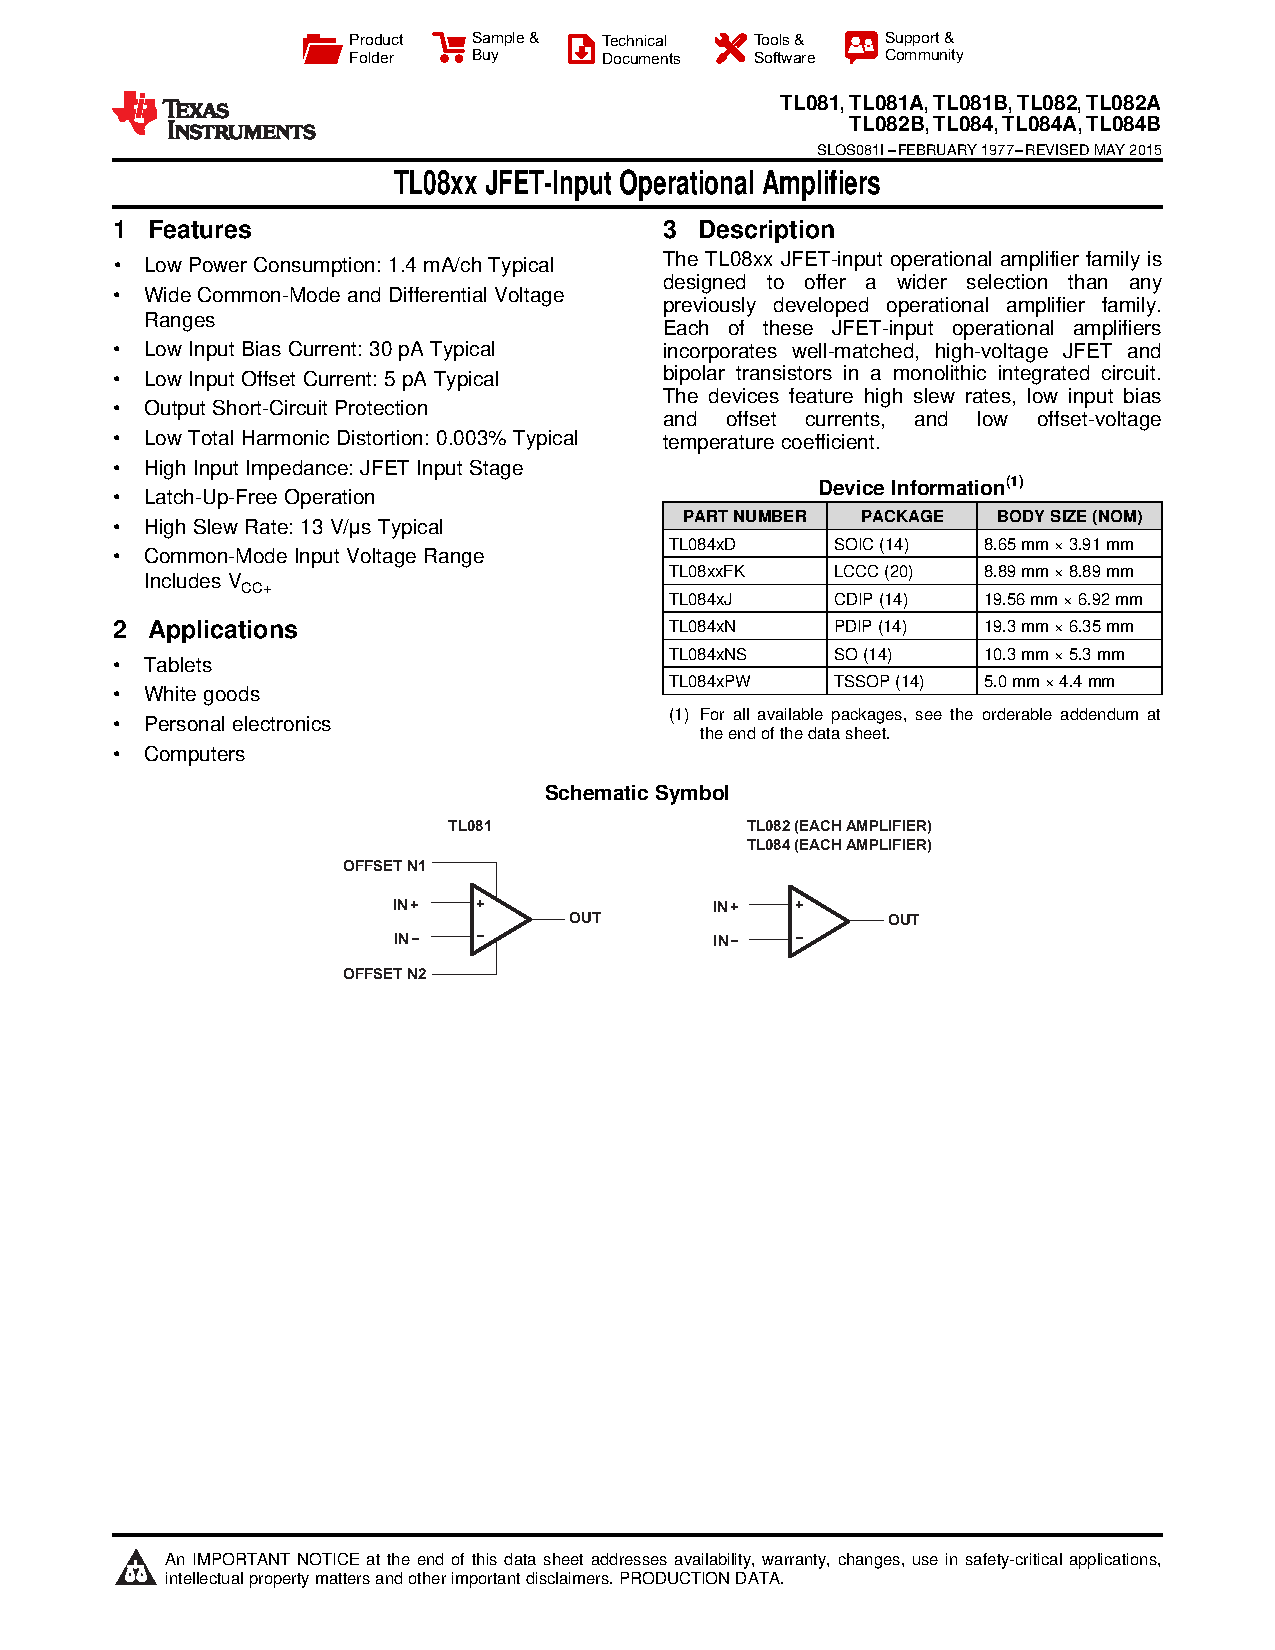
\includepdf[pages=-]{docs/doc_TL071_1p.pdf}

\end {document}